\section{可行集合上的更新}
\label{sec:feas-updates}

设$\bm{C}\subseteq\mathbb{R}^n$是非空闭凸集，$f$在包含$\bm{C}$的开集上可微，要解
\begin{equation}
 \min_{\bm{x}\in\bm{C}}f(\bm{x}).
 \label{eq:feas-problem}
\end{equation}
有了当前可行点和它的梯度，还需要关于$\bm{C}$的什么额外运算，才能算出下一个可行点？

\paragraph{三种集合运算}
梯度只描述目标，对集合一无所知。把集合的信息送进更新，最常见的有三个渠道，它们分别回答三个不同的问题。

第一种是\term{投影}（projection）：给定任意点$\bm{z}$，问$\bm{C}$中离它最近的点在哪里。第二种是线性最小化：给定方向$\bm{g}$，问$\bm{C}$中沿$-\bm{g}$走得最远的点在哪里，也就是求$\min_{\bm{s}\in\bm{C}}\langle\bm{g},\bm{s}\rangle$。第三种是用一个由集合结构决定的非欧氏尺度求“最近点”，第~\ref{sec:feas-mirror}节会定义这把尺子。

图~\ref{fig:feas-three-oracles}在预算三角形上取同一个当前点，把三种运算画在一起。投影梯度先离开集合再回来，新点落在边界上；条件梯度沿当前点与顶点的线段移动，新点是两个可行点的组合；镜像更新走一条弯曲的路径，靠近边界时自动减速。

\begin{BookInlineFigure}
  \centering
  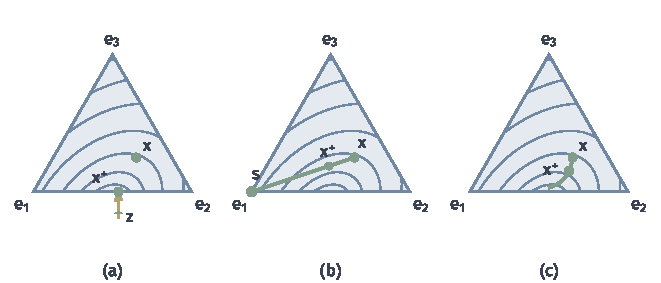
\includegraphics[width=112mm]{figures/05-optimization/06-constrained-optimization/matplotlib/feas-three-oracles/figure.pdf}
  \caption{预算三角形上从同一点$\bm{x}=(0.225,0.525,0.25)$出发的三种更新，为看清位移取较大的步长$\alpha=0.6$。(a)投影梯度：绿色箭头是平面内的梯度步，到达三角形外的空心点$\bm{z}$，黄色虚线把它拉回最近点$\bm{x}^{+}$。(b)条件梯度：线性模型在顶点$\bm{s}$处最优，新点是线段上的一点，图中取组合系数$0.25$。(c)镜像更新：绿线是步长从$0$增大时新点的轨迹，它始终留在三角形内部。}
  \label{fig:feas-three-oracles}
\end{BookInlineFigure}

\paragraph{凸性给了什么，没给什么}
$\bm{C}$凸意味着两个可行点之间的线段仍然可行。这保证条件梯度的组合可行，也保证投影存在唯一。图~\ref{fig:feas-segment-vs-curve}(a)画的就是这种情形。

凸性并不保证子问题便宜。在几千个一般线性不等式定义的多面体上，投影本身就是一个二次规划。在迹为一的半正定矩阵集合上，投影需要完整的特征分解，线性最小化却只需要一个最小特征向量。在单纯形上，投影和线性最小化都很便宜。所以选哪种方法，要先问手上的集合支持哪种运算。

\begin{BookInlineFigure}
  \centering
  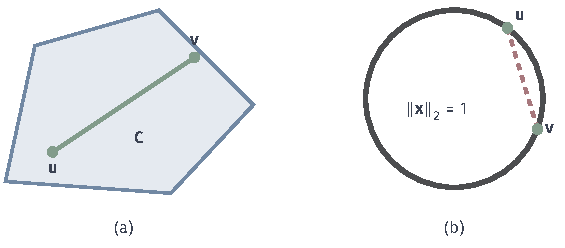
\includegraphics[width=95.75mm]{figures/05-optimization/06-constrained-optimization/tikz/feas-segment-vs-curve/figure.pdf}
  \caption{两种可行集合的差别。(a)凸集$\bm{C}$中两点$\bm{u},\bm{v}$的连线（绿色）留在集合内。(b)圆周$\lVert\bm{x}\rVert_2=1$上两点的连线（红色虚线）除端点外全部不可行，沿直线走的任何一步都要再回到圆周上。}
  \label{fig:feas-segment-vs-curve}
\end{BookInlineFigure}

\paragraph{各节使用的假设}
表~\ref{tab:feas-assumptions}列出后面各节的前提。前三行共用“集合是闭凸的”这一点，具体要求仍各不相同：条件梯度要求集合紧，否则线性子问题可能无解；镜像下降还要求势函数与集合匹配。

\begin{BookInlineTable}
  \centering
  \caption{本章各方法使用的集合、额外运算与评价量。}
  \label{tab:feas-assumptions}
  \begin{tabular}{llll}
   \toprule
   方法 & 集合 & 额外运算 & 评价量\\
   \midrule
   投影梯度 & 非空闭凸 & 欧氏投影 & 目标差、残差\\
   条件梯度 & 非空紧凸 & 线性最小化 & 目标差、间隙\\
   镜像下降 & 闭凸，配势函数 & Bregman子问题 & 平均点目标差\\
   GRG & 光滑等式加界 & 解方程 & 约束与KKT残差\\
   \bottomrule
  \end{tabular}
\end{BookInlineTable}

最后一行与前三行性质不同。图~\ref{fig:feas-segment-vs-curve}(b)的圆周不是凸集，前三种方法的保证都不能搬过去。第~\ref{sec:feas-grg}节依靠的是约束在当前点附近的局部可解性：Jacobian矩阵的一个方块要可逆，解非线性方程要能回到约束上。这些条件要逐点核对，它们失败的方式也和凸情形不同。
